% !TeX spellcheck = id_ID
\documentclass[a4paper,12pt]{article}
\usepackage[indonesian]{babel}
\usepackage{graphicx}
\usepackage{multirow}
\usepackage{enumitem}
\usepackage{listings}
\usepackage{wrapfig}
\usepackage[T1]{fontenc}
\usepackage{inconsolata}
\usepackage{lipsum}
\usepackage{adjustbox}


\usepackage{color}
\usepackage[table]{xcolor}
\definecolor{pblue}{rgb}{0.13,0.13,1}
\definecolor{pgreen}{rgb}{0,0.5,0}
\definecolor{pred}{rgb}{0.9,0,0}
\definecolor{pgrey}{rgb}{0.46,0.45,0.48}
%\lstset{language=Java,
%	showspaces=false,
%	showtabs=false,
%	breaklines=true,
%	showstringspaces=false,
%	breakatwhitespace=true,
%	commentstyle=\color{pgreen},
%	keywordstyle=\color{pblue},
%	stringstyle=\color{pred},
%	rulecolor=\color{black},
%	basicstyle=\ttfamily,
%	moredelim=[il][\textcolor{pgrey}]{$$},
%	moredelim=[is][\textcolor{pgrey}]{\%\%}{\%\%}
%}

\graphicspath{ {./img/} }
\begin{document}
\title{ {\Large Laporan Praktikum}\\ Algoritma dan Pemrograman \\{\Large Pertemuan 14}}

\author{Aldzikri Dwijayanto Prathama 
	\\195410189
	\\Teknik Informatika}
\makeatletter
\begin{titlepage}
	\begin{center}
		{\huge \bfseries \@title }\\[14ex]
		
\includegraphics[scale=.8]{logo}\\[4ex]
		{\large \@author}\\[19ex]
		{\large \bfseries {SEKOLAH TINGGI MANAJEMEN INFORMATIKA DAN KOMPUTER
				AKAKOM YOGYAKARTA}}
	\end{center}


%{\large \@date} 
\end{titlepage}
\makeatother
%\maketitle
\newpage
\tableofcontents
\newpage

\section{Tujuan}
\begin{enumerate}
    \item Mahasiswa dapat mengimplementasikan konsep Sekuensi, seleksi dan iterasi untuk menyelesaikan kasus yang sederhana
    \item Mahasiswa dapat mengubah dari satu bentuk seleksi ke bentuk seleksi yang lain begitu juga dalam perulangan
\end{enumerate}

\section{Dasar Teori}
Teori mengenai sekuensi, seleksi dan iterasi dapat dilihat pada modul pertemuan sebelumnya.

\newpage

\section{Praktik}
\subsection{Praktik 1}
Suatu rangkaian yang tersusun atas 3 resistor yang di pararel, buatlah diagram alir/flowchart yang meminta nilai R1, R2, R3 dari keyboard untuk menampilkan nilai
R dengan rumus :\\
R = 1/(1/R1+1/R2+1/R3)
\paragraph{Jawab}
\begin{center}
    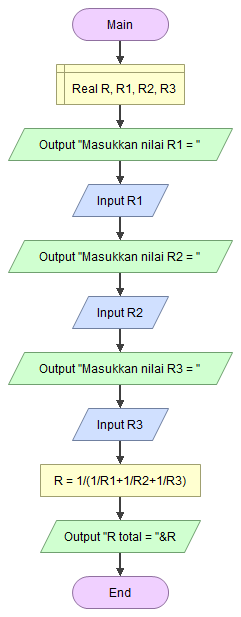
\includegraphics[height=.6\textheight]{praktik1 - Main.png}
\end{center}
Pada flowchart di atas langkah pertama adalah mendeklarasikan variabel R, R1, R2, dan R3, setelah itu menginputkan nilai dari R1, R2, dan R3. Setelah R1, R2, dan R3 mendapat nilai, selajutnya 
akan dilakukan operasi perhitungan dengan rumus R = 1/(1/R1+1/R2+1/R3). Setelah operasi perhitungan selesai, program akan mengeprint hasilnya, yang mana nilai dari operasi perhitungan tadi disimpan di variabel R.\\
Jika flowchart di atas dijalankan hasilnya seperti berikut:
\begin{center}
    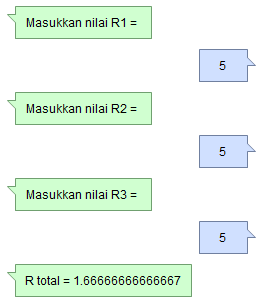
\includegraphics[scale = 1]{main1.PNG}
\end{center}

\subsection{Praktik 2}
Buat program untuk menghitung nilai R berdasarkan kasus praktik 1
\paragraph{Jawab}
\begin{center}
    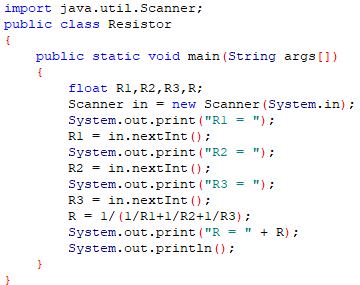
\includegraphics[width = 0.8\linewidth]{prak2.PNG}
\end{center}
Program java di atas memiliki algoritma yang sama dengan flowchat di praktik 1. Agar program dapat memasukkan input dari user dibutuhkan modul Scanner, setelah itu dideklarasikan variabel new
sebagai scanner, dan R, R1, R2, dan R3 sebagai variabel float karena pada operasi penghitungan nanti terdapat kemungkinan hasilnya adalah bilangan pecahan. Setelah itu terdapat fungsi untuk
memasukkan nilai variabel dari user saat program dijalankan. Setelah R1, R2, dan R3 mendapat niai, dilakukan
operasi perhitungan dengan rumus R = 1/(1/R1+1/R2+1/R3), setelah penghitungan selesai program akan mengeprint variabel R, yang menyimpan hasil perhitungan tadi.\\
Output dari program tersebut seperti berikut:
\begin{center}
    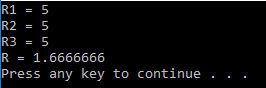
\includegraphics[scale = 1, width=0.8\linewidth]{prak2b.PNG}
\end{center}

\newpage
\subsection{Praktik 3}
Buatlah flowchart dan program untuk menghitung nilai rata-rata dari minimal 5 data yang dimasukan menggunakan keyboard
\paragraph{Jawab}
\begin{center}
    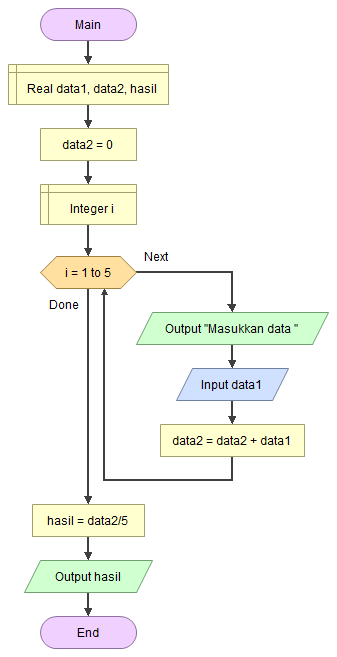
\includegraphics[scale = 0.8]{praktik3 - Main.png}
\end{center}
Pada flowchart di atas variabel data1, data2, dan hasil dideklarasikan sebagai real terlebih dahulu, lalu data 2 diberi nilai 0, setelah itu dideklarasikan integer i. 
Selanjunya dibawahnya kita beri looping for, variable-nya kita isi dengan i, Start Value isi dengan 1 dan End Value kita isi dengan 5.
Di dalam perulangan for terdapat operasi untuk memasukkan angka dan menjumlahkan semua angka yang dimasukkan, dan memasukkan hasilnya ke variabel data2, setelah perulangan selesai variabel
data2 akan dibagi 5, dan hasilnya akan disimpan ke variabel hasil. Lalu program akan mengeprint variabel hasil.\\
Jika flowchart dijalankan akan menjadi seperti berikut:
\begin{center}
    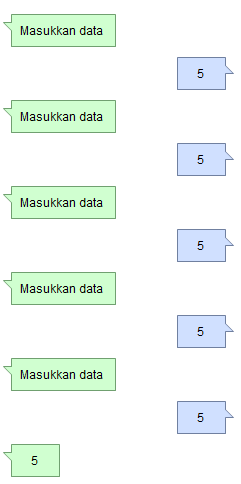
\includegraphics[scale = 0.8]{praktik3.PNG}
\end{center}
Selanjutnya adalah membuat program java dengan algoritma seperti flowchart di atas
\begin{center}
    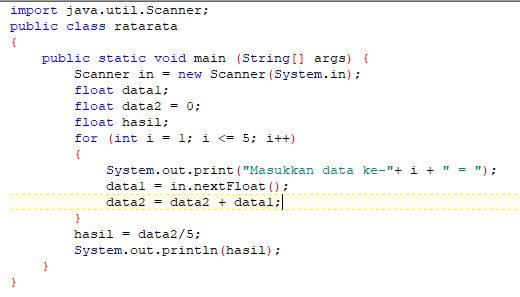
\includegraphics[scale = 0.8]{prak3.PNG}
\end{center}
Sama seperti flowchart sebelumnya program java ratarata di atas memiliki perulangan for, yang diulang sebanyak 5 kali, didalamnya terdapat pernyataan untuk memberi nilai ke variabel data1, dan
menjumlahkan semua bilangan yang dimasukan dan memasukkan hasilnya ke variabel data2. Setelah perulangan selesai nilai di variabel data2 akan dibagi dengan 5. Lalu program akan mengeprint
variabel hasil.\\
Jika program dijalankan maka outputnya seperti berikut:
\begin{center}
    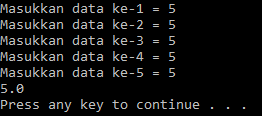
\includegraphics[scale = 0.8]{prak3b.PNG}
\end{center}

\subsection{Praktik 4}
Modifikasi praktik 3 agar jumlah data yang akan dihitung rata-ratanya bisa fleksibel sesuai keinginan user
\paragraph{Jawab}
\begin{center}
    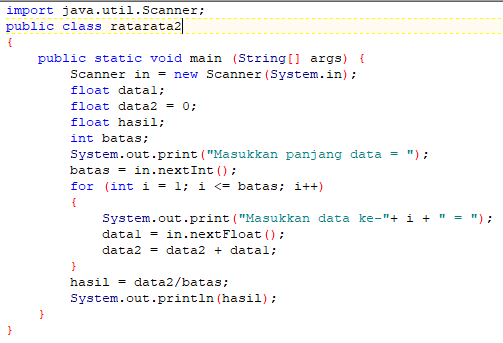
\includegraphics[scale = 0.8]{prak4.PNG}
\end{center}
Agar program dari praktik 3 bisa dimasukkan data sebanyak yang diperlukan user, ditambahkan variabel batas yang akan ditentukan oleh user. Kondisi pada perulangan for i<=5 diganti menjadi
i<=batas, sehingga bisa dimasukkan data sebanyak nilai pada variabel batas. setelah itu nilai pada variabel data2 dibagi dengan nilai pada variabel batas.

\section{Latihan}
Pada latihan pertemuan ini kita akan mengetikkan program untuk membuat Segitiga bintang Terbalik.
\begin{center}
    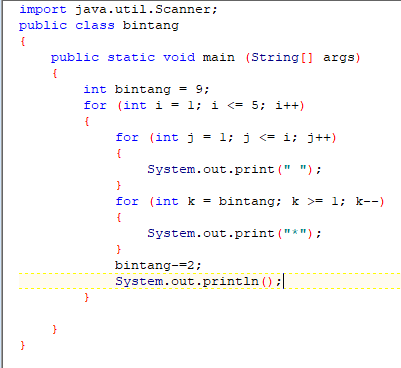
\includegraphics[scale = 0.8]{latihan.PNG}
\end{center}
Program java diatas terdapat perulangan di dalam perulangan, induk perulangan berfungsi untuk mengeprint newline, didalamnya terdapat dua perulangan. Perulangan pertama berfungsi untuk spasi, 
untuk baris ke 1 tidak mengeprint spasi, untuk baris ke 2 akan mengeprint 1 spasi, dan seterusnya, sehingga jika nanti ditambahkan *, posisinya akan berada di tengah. Perulangan kedua berfungsi untuk mengeprint bintang. Setalah itu terdapat pernyataan untuk mengurangi nilai di variabel bintang dengan 2, sehingga semakin ke bawah jumlah bintang akan semakin sedikit.
Jadi jika program dijalankan akan membentuk segitiga terbalik bintang seperti berikut:
\begin{center}
    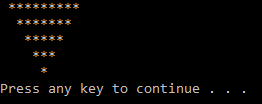
\includegraphics[scale = 0.8]{latihanb.PNG}
\end{center}

\newpage
\section{Tugas}
Pada tugas ini kita akan membuat program untuk menghitung akar-akar persamaan kuadrat(diskriminan) dimana memiliki akar penyelesaian berupa x1 dan x2, dengan ketentuan:
\begin{itemize}
    \item Jika diskriminan lebih besar daripada 0, kedua nilai x yang menjadi solusi persamaan tersebut berupa bilangan real.
    \item Jika diskriminan sama dengan nol, kedua nilai x yang menjadi solusi persamaan tersebut berupa bilangan kembar.
    \item Jika diskriminan lebih kecil dari pada nol, kedua nilai x yang menjadi solusi persamaan tersebut berupa bilangan kompleks
\end{itemize}
\begin{center}
    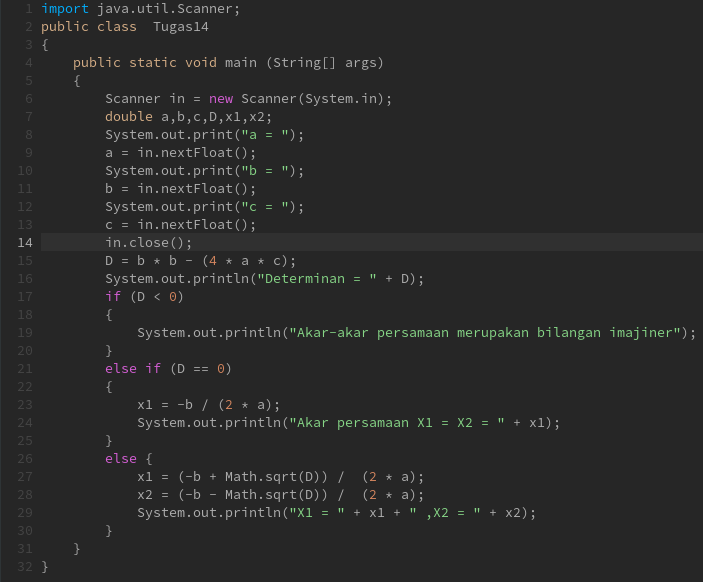
\includegraphics[scale = 0.6]{tugas.png}
\end{center}
Pada program di atas dideklarasikan variabel a, b, c, D, x1, dan x2 sebagai double. Lalu terdapat pernyataan input untuk nilai a, b, dan c. Jika variabel a, b, dan c sudah dimasukkan nilai
akan dilakukan operasi penghitungan dengan rumus diskriminan yaitu b * b - 4ac
selanjutnya terdapat seleksi if dengan kondisi D kurang dari 0 dengan output dibawahnya. Baris selanjutnya kita beri else if dengan kondisi D sama dengan 0,
dibawahnya kita beri rumus untuk mencari nilai X1nya dan juga kita beri perintah untuk menampilkan outputnya. Pada else kita beri dua rumus untuk X1 dan X2 dengan rumus
$x = \frac {−b \pm \sqrt{b^{2}} − 4ac}{2a}$
. Pada baris selanjutnya
kita beri perhitungan akar kuadrat yang dapat dilakukan dengan fungsi sqrt().
Fungsi ini terdapat dalam class Math. Jadi untuk menghitung akar seperti di
atas dalam kode java dapat dilakukan dengan cara menuliskan Math.sqrt();.
Kemudian pada baris berikutnya baru kita beri output untuk nilai X1 dan X2nya.\\
Output jika program dijalankan akan seperti berikut:
\begin{center}
    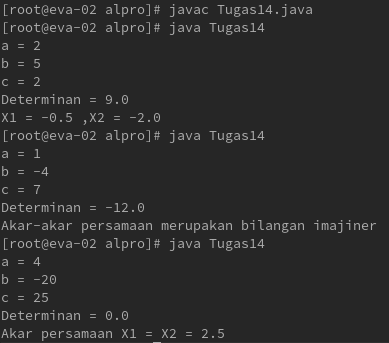
\includegraphics[scale = 0.8]{tugasb.png}
\end{center}

\newpage
\section{Kesimpulan}
lebih memahami tentang konsep
Sekuensi, seleksi dan iterasi untuk menyelesaikan kasus yang sederhana dan
dapat mengubah dari satu bentuk seleksi ke bentuk seleksi yang lain begitu juga
dalam perulangan.
\end{document}
